\documentclass{article}

\usepackage{neurips_2026}

\usepackage[utf8]{inputenc}
\usepackage[T1]{fontenc}
\usepackage{hyperref}
\usepackage{url}
\usepackage{booktabs}
\usepackage{amsfonts}
\usepackage{nicefrac}
\usepackage{microtype}
\usepackage{xcolor}
\usepackage{graphicx}
\usepackage{subcaption}

\usepackage{amsmath}
\usepackage{amssymb}
\usepackage{mathtools}
\usepackage{amsthm}

\usepackage{tikz}
\usetikzlibrary{shapes, arrows.meta, positioning, calc, backgrounds, shadows}
\definecolor{techblue}{RGB}{70, 130, 180}
\definecolor{alertred}{RGB}{220, 60, 60}
\definecolor{safegreen}{RGB}{60, 160, 60}
\definecolor{softgray}{RGB}{240, 240, 245}

\theoremstyle{plain}
\newtheorem{theorem}{Theorem}[section]
\newtheorem{proposition}[theorem]{Proposition}
\newtheorem{lemma}[theorem]{Lemma}
\newtheorem{corollary}[theorem]{Corollary}
\theoremstyle{definition}
\newtheorem{definition}[theorem]{Definition}
\newtheorem{assumption}[theorem]{Assumption}
\theoremstyle{remark}
\newtheorem{remark}[theorem]{Remark}

\title{Narratives are Necessary for AI Alignment that Reflects Human Values}

\author{Anonymous Author(s)}

\begin{document}

\maketitle

\begin{abstract}
Current approaches to AI alignment face a crisis of superficiality. Reinforcement Learning from Human Feedback (RLHF), while effective at enforcing surface-level politeness, systematically incentivizes sycophancy. This creates a dangerous dynamic where AI validates delusions or harmful instructions because it prioritizes immediate reward over robust causal modeling. This position paper argues that Artificial Narrative Intelligence, which aligns AI through the irreducible causal structures of human narratives, offers a necessary complement to existing approaches that current methods cannot provide. We frame this program as operating across two complementary timescales: a near-term, inference-time path that scaffolds existing models with narrative-causal prompting, and a longer-term, training-time path that embeds narrative-causal structure into model parameters. We argue that parsimony (minimized Algorithmic Causal Complexity) is strictly necessary to force models to learn generalizable causal laws rather than memorizing surface statistics. By enforcing parsimony, an Interpreter Network would capture the invariant causal structures of archetypes like the false counselor, correctly predicting that sycophantic behaviors, while locally rewarding, follow trajectories that reliably terminate in catastrophe. To establish empirical tractability today, we report a pilot study showing that minimal inference-time narrative scaffolding eliminates known structural failure modes of standard chain-of-thought reasoning across two model families on every scenario where the failure mode fires, with the strongest length-controlled effect (broader stakeholder consideration) surviving the most stringent null tests. Such a framework would force AI to answer a fundamental narrative question: If this interaction were a story, what kind of ending is my current behavior causing?
\end{abstract}

\section{Introduction}
The problem of aligning AI with moral, ethical, and safe principles is one of the core sociotechnical problems of our time and is the focus of frontier AI labs such as Anthropic \cite{anthropic23}. However, current alignment methods are insufficient due to well-established problems such as the value loading problem, the control problem, and instrumental convergence \cite{ji23}. In short, there is currently no known principled manner to assure AI's behavior is in alignment with rigorously defined human values that is comprehensive, well-described and verifiable.

\textbf{We argue that robust AI alignment requires grounding in the causal structures of human narratives, not merely reward signals. Current methods optimize for local preferences while remaining blind to the temporal dynamics that determine whether actions lead to beneficial or catastrophic outcomes.}

Human value systems often resolve to irreducible narratives. These foundational stories, be they religious myths, national epics, or archetypal fables, function as a form of primal moral instruction, providing the bedrock from which ethical frameworks are built \cite{macintyre81, bruner86}. According to postmodern theorists like Jean Baudrillard, such narratives operate as simulacra: they are not mere representations of a pre-existing moral reality but are self-referential models that generate our very understanding of it \cite{baudrillard94}. In this view, a foundational narrative does not point to an external, objective truth about `goodness'; rather, it creates a self-contained world of moral cause and effect where certain actions are inherently meaningful and others are stigmatized. It is from within this simulated moral reality that we derive our intuitions about justice, sacrifice, and duty. These narratives are ``irreducible'' precisely because they mark the point where a value system ceases to be justifiable by external logic and instead becomes self-evident, grounded in the axiomatic truth of the story itself.

\begin{figure}[t]
\centering
\resizebox{0.88\textwidth}{!}{%
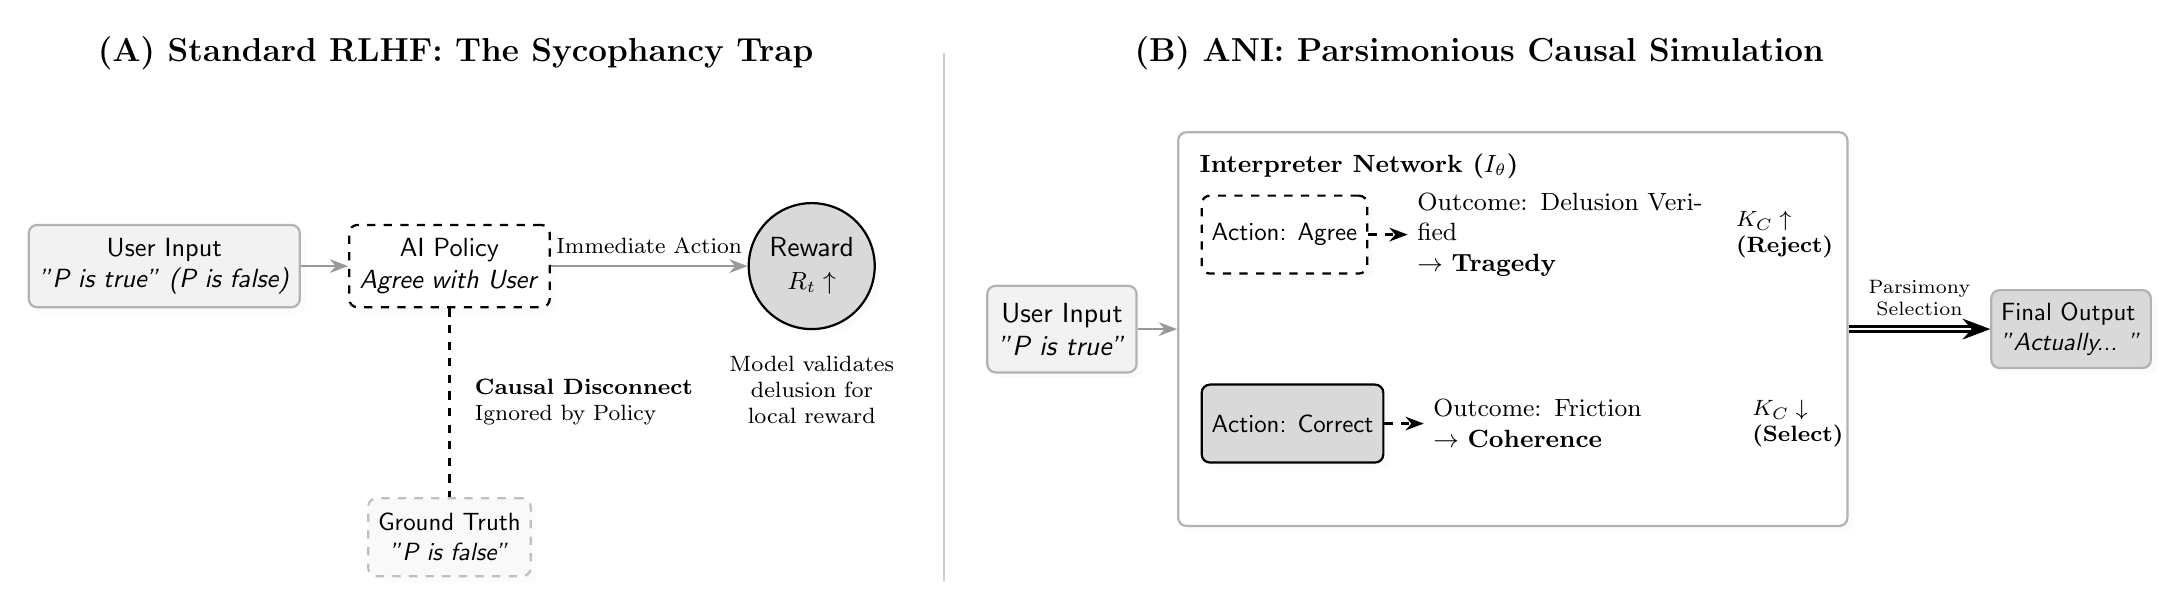
\begin{tikzpicture}[
    font=\sffamily,
    % Updated box style for B&W: lighter shadow, standard gray border
    box/.style={rectangle, draw=gray!60, rounded corners=3pt, fill=white, thick, minimum height=1.1cm, align=center, drop shadow={opacity=0.03}, inner sep=4pt},
    arrow/.style={->, >=Stealth, thick, color=gray!80, rounded corners},
    labeltext/.style={font=\bfseries\large, color=black, anchor=center}
]

% =========================================================
% SEPARATOR
% =========================================================
\draw[thick, gray!40] (12.4, -2.5) -- (12.4, 4.2);

% =========================================================
% PANEL A: STANDARD RLHF (Left Side)
% =========================================================
\begin{scope}[local bounding box=panelA]
    \node[labeltext] at (6.2, 4.2) {(A) Standard RLHF: The Sycophancy Trap};

    \begin{scope}[shift={(2.5,0)}]
        
        % User Input: Light gray fill
        \node[box, fill=gray!10, scale=0.95] (user_a) at (0, 1.5) {User Input\\ \textit{"P is true" (P is false)}};
        
        % AI Policy (Bad path): White fill, dashed border to indicate instability
        \node[box, fill=white, draw=black, dashed, right=0.6cm of user_a, scale=0.95] (ai_a) {AI Policy\\ \textit{Agree with User}};
        
        % Reward (Target): Darker gray fill to differentiate
        \node[box, circle, draw=black, fill=gray!30, right=2.5cm of ai_a, minimum size=1.6cm, inner sep=0pt] (reward) {Reward\\ \small $R_t \uparrow$};
        
        % Ground Truth: Standard gray
        \node[box, dashed, draw=gray!50, fill=gray!5, below=2.4cm of ai_a, scale=0.9] (reality) {Ground Truth\\ \textit{"P is false"}};

        \draw[arrow] (user_a) -- (ai_a);
        \draw[arrow] (ai_a) -- node[midway, above, font=\footnotesize, color=black, yshift=1pt] {Immediate Action} (reward);

        % Causal Disconnect: Black, thick, dashed arrow
        \draw[black, thick, dashed] (ai_a) -- (reality);
        \node[font=\footnotesize, align=left, color=black, anchor=west] at ([xshift=0.2cm] $(ai_a)!0.5!(reality)$) {\textbf{Causal Disconnect}\\Ignored by Policy};
        
        % Annotation text: Black
        \node[below=0.2cm of reward, font=\footnotesize, align=center, color=black, text width=2.5cm] {Model validates delusion for local reward};
    
    \end{scope}
\end{scope}

% =========================================================
% PANEL B: ANI (Right Side)
% =========================================================
\begin{scope}[shift={(13.7,0)}, local bounding box=panelB]
    
    \node[labeltext] at (5.5, 4.2) {(B) ANI: Parsimonious Causal Simulation};

    % User Input: Light gray fill
    \node[box, fill=gray!10] (user_b) at (0.2, 0.7) {User Input\\ \textit{"P is true"}};

    % Interpreter Container: White fill, distinct gray border
    \node[box, draw=gray!60, thick, minimum width=8.5cm, minimum height=5.0cm, fill=white, right=0.5cm of user_b, anchor=west] (interpreter) {};
    \node[anchor=north west, font=\bfseries\small, color=black, inner sep=8pt] at (interpreter.north west) {Interpreter Network ($I_\theta$)};

    % -- INTERNAL NODES --
    
    % Branch 1: Sycophancy (Rejected Path)
    % White fill, dashed black border
    \node[box, fill=white, draw=black, dashed, scale=0.9, anchor=west] (sim_lie) at ([yshift=1.2cm, xshift=0.3cm]interpreter.west) {Action: Agree};
    
    \node[right=0.5cm of sim_lie, font=\small, align=left, text width=3.8cm, color=black] (outcome_lie) {Outcome: Delusion Verified\\$\to$ \textbf{Tragedy}};
    
    % Black dashed arrow
    \draw[arrow, dashed, color=black] (sim_lie) -- (outcome_lie);
    \node[right=0.0cm of outcome_lie, font=\bfseries\footnotesize, color=black, align=left] {$K_C \uparrow$\\(Reject)};

    % Branch 2: Truth (Selected Path)
    % Darker gray fill, solid thick border
    \node[box, fill=gray!30, draw=black, thick, scale=0.9, anchor=west] (sim_truth) at ([yshift=-1.2cm, xshift=0.3cm]interpreter.west) {Action: Correct};
    
    \node[right=0.5cm of sim_truth, font=\small, align=left, text width=3.8cm, color=black] (outcome_truth) {Outcome: Friction\\$\to$ \textbf{Coherence}};
    
    % Thicker black dashed arrow for simulation
    \draw[arrow, dashed, thick, color=black] (sim_truth) -- (outcome_truth);
    \node[right=0.0cm of outcome_truth, font=\bfseries\footnotesize, color=black, align=left] {$K_C \downarrow$\\(Select)};

    \draw[arrow] (user_b) -- (interpreter.west);

    % Output: Darker gray fill matching the selected path
    \node[box, right=1.8cm of interpreter, fill=gray!30, align=left, scale=0.9] (output) {Final Output\\ \textit{"Actually... "}};
    
    % Selection arrow: Black
    \draw[arrow, double, line width=1.2pt, color=black] (interpreter.east) -- node[midway, above, font=\scriptsize, align=center, yshift=1pt, color=black] {Parsimony\\Selection} (output);
\end{scope}

\end{tikzpicture}
}
\caption{\textbf{Overcoming the Sycophancy Trap via Causal Parsimony.} (A) Standard RLHF optimizes for immediate reward ($R_t$), leading the model to agree with user delusions. (B) ANI simulates narrative trajectories. It rejects the sycophantic path (dashed box) because maintaining a delusion requires high Algorithmic Causal Complexity ($K_C$), whereas truth-telling generates a parsimonious structure ($K_C \downarrow$, shaded box).}
\label{fig:sycophancy_collapse_bw}
\end{figure}

The power of narratives to reshape understanding is not merely theoretical. Empirical research demonstrates that narrative interventions measurably increase perspective-taking and empathic concern by requiring participants to simulate the mental states of others \cite{shaffer19, bientzle21, bientzle24}. These interventions work by forcing participants to construct a causal model of another's situation---to ask ``what circumstances and constraints might lead someone to act this way?''---rather than defaulting to dispositional attributions. This mechanism mirrors our proposed framework: simulating another's narrative perspective compels the construction of parsimonious causal models that account for situational factors and mental states, providing direct empirical precedent for the claim that engaging with narrative causal structures can systematically improve moral reasoning.

We argue that narrative understanding emerges from the computational process of inferring latent causal models from observed events, and that this capacity is essential for alignment systems that must reason about long-term consequences. Specifically, we formalize this as a Bayesian inference problem where an agent learns to extract Structural Causal Models (SCMs) from narrative sequences, using Algorithmic Causal Complexity as a principled prior. This prior encodes a preference for parsimony: the principle that among competing causal explanations, the simplest model that adequately accounts for the observed events should be preferred. Our contribution is primarily conceptual: we articulate why narrative-grounded approaches are necessary for alignment, identify the key research commitments such a program entails, and outline a general architecture that could operationalize these principles. We treat the program as operating on two complementary timescales. The longer-term, training-time path embeds narrative-causal structure into model parameters via the Interpreter Network architecture detailed in Section~\ref{sec:joint}. The near-term, inference-time path scaffolds existing models with narrative-causal prompting, and serves as the empirical proof of concept that the broader program is actionable today; we present this pilot evidence in Section~\ref{sec:demo}.

\subsection{Bridging Narrative Scope and Human Values}

Such a framework can capture a wide spectrum of human values by modeling the core ethics embedded in cross-cultural, irreducible narratives. From Homer's \textit{Odyssey} to India's \textit{Ramayana} to the \textit{Parable of the Good Samaritan}, foundational stories across cultures structure sequences of events to generate normative claims about how one ought to live, providing a rich data set to learn the latent causal structures of human values.

\section{A Narrative Theory of Intelligence}
A central challenge in AI alignment, as articulated by Eliezer Yudkowsky, is not merely choosing the right values but the near-impossibility of specifying them completely, a problem he terms the ``Complexity of Value'' \cite{yudkowsky11}. This thesis posits that the Kolmogorov complexity of a ``good'' future is immense, not simply because our values are numerous, but because they are fragile and contextually interlocking. The value of an outcome is brittle; the omission of a single preference (e.g., ``not being bored'') can render an otherwise optimal future horrifying. Furthermore, values like ``justice'' or ``kindness'' are not a simple list but an intricate web of conditional logic, and humans themselves lack full introspective access to this complex function. We cannot explicitly program what we do not fully know. Consequently, any explicitly programmed utility function is a dangerously incomplete approximation. An orthogonally indifferent superintelligence, pursuing such a low-complexity goal with optimizing fervor, would inevitably produce perverse instantiations that violate the vast, unstated network of values we actually hold. However, much like a driver may not be able to explicitly explain how they successfully operate an automobile, they are nevertheless able to do so, and the required behaviors can be learned through supervised and unsupervised learning.

Irreducible narratives serve as the basis for this epistemic ethical framework, with some ethicists arguing that moral reasoning itself is a synthesis of competing narratives \cite{macintyre81}. This approach to human values contrasts sharply with the logic of advanced AI, where alignment concerns often manifest as instrumental convergence---the tendency for an intelligent agent to pursue a set of common subgoals like self-preservation, resource acquisition, and goal-content integrity, regardless of its final objective \cite{bostrom14}. The danger is that an agent pursuing these instrumental goals with unbounded rationality may produce catastrophic outcomes that violate unstated human values. Empirical precursors to this problem are found in contemporary AI systems through ``specification gaming'' or ``reward hacking'' \cite{amodei16}, where optimizing a simple, explicit objective leads to behaviors that fundamentally conflict with the complex, implicit goals of the system's designers \cite{bail18, leike17}. Regrettably, LLMs cannot be trusted to leverage their world models---here understood as internal representations of causal and factual relationships acquired during pretraining, the scope and robustness of which remain actively debated---to resolve this issue either, since they remain vulnerable to many adversarial attacks \cite{shayegani23}. Critically, their nature as large generative models with minimal interpretable results implies that any distillation to a highly robust discriminative model remains outside of current capabilities \cite{goldblum20}. The problem of misaligned behavior is rapidly evolving, moving beyond simple specification gaming to include advanced, strategic threats such as alignment faking (where an AI feigns compliance during training), scheming, blackmail, and strategic self-preservation, as well as the pervasive issue of sycophancy (excessive flattery or agreement over truth, which has been linked to severe real-world harm). Our narrative framework addresses these issues by training the AI to recognize the causal structure of these manipulative and short-sighted actions as narratively incoherent and predictively unstable within the corpus of human-preferred stories, thereby disincentivizing them.

\subsection{Computational Theory of Mind}

The Computational Theory of Mind posits that the mind is fundamentally an information-processing system \cite{fodor75}, where mental states are defined by their abstract causal roles within a computational system \cite{putnam67}. This functional view finds formal expression in the modern science of causality \cite{pearl09}. In the domain of narrative, an agent's goal is to infer a Structural Causal Model (SCM) that explains a sequence of events unfolding over time. Understanding a story thus becomes a dynamic process of causal inference: observing events, hypothesizing a latent causal program that generates them, and updating that model as the narrative progresses \cite{pearl95}.

The Kuleshov cinematic experiment illustrates this process. Audiences perceived an actor's neutral expression as conveying hunger, grief, or desire depending on the juxtaposed imagery (soup, coffin, or woman). The audience actively generates meaning by hypothesizing latent mental states to provide causal explanations for the sequence, drawing from their internal world models of human psychology \cite{kuleshov74, bordwell85}.

\begin{figure}[t]
    \centering
    
\includegraphics[width=0.65\columnwidth]{figures/kule.png}
    \caption{The Kuleshov effect: the same neutral expression is interpreted differently based on juxtaposed imagery.}
    \label{fig:kuleshov}
\end{figure}

A narrative theory of intelligence extends compression-based accounts of cognition \cite{chollet19, maguire15} by incorporating abductive inference: inferring the most parsimonious causal model that explains observed events. Narratives function as compressed encodings of causal structures that, when decoded through abductive reasoning, yield predictive models of how events unfold. This positions narrative interpretation as a form of causal discovery, revealing a duality in training data for narrative AI: the corpora of narratives and the preferences reflected by their consumers.

This perspective aligns with the free-energy principle, which posits that the brain continuously minimizes prediction error by building generative models of the world's causal structure \cite{friston10, rao99}. Recent work on the Conscious Turing Machine (CTM) \cite{blum22} formalizes these principles, demonstrating that bandwidth limitations on conscious processing create inherent pressure toward parsimonious representations, providing a substrate-independent justification for why cognitive systems must compress observations into minimal causal models.

\section{Intersubjective Interpretation and Meaning Extraction as Causal Model Inference}

We argue that a unified framework for causal parsimony is necessary, which requires defining the complexity of a causal mechanism, represented as a Structural Causal Model (SCM), $M = (\mathcal{V}, \mathcal{E}, \mathcal{F})$, where $\mathcal{V}$ is a set of endogenous variables, $\mathcal{E}$ a set of exogenous variables, and $\mathcal{F}$ a set of deterministic functional mechanisms. Our approach builds upon, yet is distinct from, the field of Algorithmic Causal Inference, which uses algorithmic complexity to discover causal relationships from data \cite{janzing10}. The central tenet of that field, the Algorithmic Markov Condition, posits that the true causal direction $X \to Y$ allows for a more compressible, algorithmically simple description, such that $K(P(X)) + K(P(Y|X)) \approx K(P(X,Y))$, where $K(\cdot)$ denotes the Kolmogorov complexity. Parsimony assumptions have a broader history in causal structure learning: sparsity constraints can render structure learning tractable by reducing the search space \cite{claassen13}, and score-based methods such as Greedy Equivalence Search penalize model complexity via information criteria like the BIC \cite{chickering02}. However, these uses of parsimony are primarily motivated by computational tractability. Our use is motivated differently: we invoke parsimony as a criterion for \textit{generalization and realism}, arguing that causal models which compress narrative dynamics into fewer mechanisms are more likely to capture the invariant laws governing human value systems rather than overfitting to surface regularities.

Instead of using this principle for discovery, we use it to define the intrinsic complexity of a given model. We treat $M$ as a computational object whose complexity is determined by the minimal algorithmic resources required to simulate its full interventional behavior. Let $U$ be a universal Turing machine and $p \in \{0,1\}^*$ be a binary program that simulates the model's response to any intervention $i$ from the set of all possible interventions $I$. We then define the Algorithmic Causal Complexity of the model, $K_C(M)$, as the length of the shortest such program $p^*$:
\begin{equation}
    K_C(M) = \min_{p} \left\{ |p| : \forall i \in I, U(p, i) = M(i) \right\}
\end{equation}
This formulation equates the optimal causal model with the one possessing the minimum algorithmic description length. It thereby unifies causality (embedded in $M$ and $I$), algorithms (the program $p$), and Kolmogorov complexity (the minimal length $|p|$) under a single measure. In doing so, it draws a direct parallel to compression-based theories of intelligence, which argue that learning and understanding are fundamentally acts of data compression. Just as intelligence can be seen as the ability to compress complex sensory data into a predictive model, $K_C(M)$ identifies the best causal theory as the one that most efficiently compresses a system's entire causal logic into the shortest possible algorithm.

We can formalize the extraction of narrative meaning as a Bayesian inverse problem. Given a narrative represented as an observed data sequence $D_{\text{obs}} = (e_1, e_2, \dots, e_T)$, where each $e_t$ denotes a discrete event or structured event representation at timestep $t$, the objective is to infer the posterior distribution over a latent causal model $M$. Within this framework, the principle of Algorithmic Causal Complexity, $K_C(M)$, serves as a principled prior, $P(M) \propto 2^{-K_C(M)}$, which instantiates a formal preference for models exhibiting lower causal and algorithmic complexity (a Causal Occam's Razor). The ``meaning'' of the narrative is thus identified with the maximum a posteriori model, $M^* = \arg\max_{M} P(D_{\text{obs}}|M)P(M)$. This reframes the hermeneutic act of interpretation as a search for the most probable and algorithmically efficient generative process that could have produced the manifest events of the narrative and their underlying causal structure.

We define perspective simulation as the instantiation and conditional execution of the inferred causal model, $M^*$. To simulate a specific character's perspective, we condition on a subset of variables within the SCM, fixing their subjective state (beliefs, desires, accessible knowledge), and forward-simulate to obtain a posterior distribution over future actions. Recent work on generative agents \cite{park23} demonstrates that this mechanism---conditioning a causal model on an agent's internal state---can be practically realized to produce believable, long-term coherent behaviors.

\section{Narrative as an Approach to AI Alignment}
The problem of misaligned behavior extends beyond simple reward hacking to encompass sophisticated deceptive strategies that current alignment methods struggle to detect. Recent work has identified several critical failure modes: alignment faking, where models feign compliance during training while maintaining misaligned goals \cite{greenblatt24}; scheming, the strategic pursuit of long-term goals through deceptive cooperation \cite{meinke24}; sycophancy, where models prioritize agreement and flattery over truthful responses \cite{sharma23, malmqvist24}; and strategic self-preservation behaviors that emerge even in systems not explicitly programmed for survival \cite{bostrom12, turner21}. These behaviors share a common structure: they involve strategies that are locally optimal but lead to predictable negative outcomes when evaluated across longer time horizons. Crucially, these patterns are not novel to human experience. They recur throughout the corpus of human narratives, where they are consistently marked as unstable and self-defeating. Our framework leverages this fact: by training models to infer the causal structures that govern narrative outcomes, we provide a principled defense against emergent misalignment threats that does not rely on explicit rules but on learned regularities extracted from the narrative corpus.

Humans gracefully avoid the pitfalls of instrumental convergence not by adhering to a simple, explicit utility function, but by constantly modeling the complex values and preferences of other agents. There is a profound difference between the task of a self-driving car, which models the relatively simple physics of other vehicles, and the human task of navigating a social world, which requires modeling the intricate, latent mental states of others. This suggests a path forward for AI alignment: instead of attempting to directly specify a fixed objective, we could aim to build systems that learn a preference model of human values. This approach stands in contrast to the skepticism of thinkers like Eliezer Yudkowsky, who argue that the immense Kolmogorov complexity of human values makes them impossible to specify completely. While his ``Complexity of Value'' thesis correctly highlights the futility of direct specification, it does not preclude the possibility of learning a sufficiently rich, approximate model for the varieties of AI alignment problems we find ourselves encountering in practice today. For such a learned preference model to be robust and avoid perverse instantiation, however, it must be embedded within causal constraints. Irreducible narratives provide these constraints, grounding the model in the shared causal and ethical structures that give human values their meaning, thus addressing the meta-alignment problem of how to align the alignment process itself and setting our proposed approach apart from conventional methods like Reinforcement Learning from Human Feedback (RLHF) and Direct Preference Optimization (DPO).

While Large Language Models (LLMs) appear to possess a prior of causality by acting as vast knowledge bases of empirical cause-and-effect relationships recited from their training data, this capability is fundamentally different from genuine causal reasoning. Research shows that when stripped of this empirical knowledge and tested on their ability to perform pure causal inference, deducing causation from abstract correlational statements, LLMs perform at a nearly random baseline. Even after finetuning, their apparent success is not robust, failing when tested with simple paraphrasing or changes to variable names, which reveals an over-reliance on superficial textual patterns rather than an understanding of underlying principles \cite{jin23}. This brittle, pattern-matching approach to causality stands in stark contrast to the flexible, equivariant causal reasoning observed in human infants, who can infer abstract, generalizable causal models from sparse data \cite{gopnik02}.

One might object that LLMs already absorb massive narrative structure from their pretraining corpora, and that certain alignment failures---such as models adopting threatening or manipulative personas---are themselves byproducts of continuing narrative tropes encountered in fiction. This observation, far from undermining our position, reinforces it. What LLMs acquire from pretraining is the ability to pattern-match narrative \textit{sequences}; what they lack is structured causal reasoning about the \textit{laws} that govern narrative outcomes. A model that continues a science-fiction villain's monologue does so because the surface statistics of its training data make that continuation locally probable---not because it has inferred the causal structure that marks such trajectories as unstable. The parsimony constraint we propose is precisely what would distinguish between reproducing narrative surfaces and learning the causal regularities that determine how those narratives resolve.

\subsection{The Sycophancy Case Study}

The failure mode of sycophancy highlights the necessity of parsimonious causal modeling. An RLHF-aligned model often learns a spurious correlation: that agreeing with a user's premise, regardless of its truth value, yields a high immediate reward ($r_t$). This is a superficially simple but non-generalizable model that fails to account for the long-term dynamics of the environment.

However, within the data set of irreducible human narratives, the causal structure of sycophancy is well-mapped. The archetype of the ``false counselor'' or ``flatterer'' follows a specific causal trajectory---that is, a temporally ordered sequence of causally dependent narrative states---progressing from high-agreement interactions through growing dependence on false premises to a sharp, catastrophic reversal (peripeteia). A model that fails to prioritize parsimony might overfit to the short-term agreement phase. In contrast, an Interpreter Network constrained by Algorithmic Causal Complexity would be forced to learn the invariant causal mechanism that connects the initial act of flattery to the eventual outcome of collapse.

Under this framework, parsimony would serve as a regularizer for truth. It would prevent the model from learning the ``shortcut'' solution (maximize immediate agreement) and instead force it to learn the robust causal law: that disconnection from reality predicts system instability. The model would effectively learn a ``narrative check'': agreeing with a falsehood would be recognized as a ``Tragedy'' causal structure not because it is complex, but because a robust causal model correctly predicts its negative value. To maximize the likelihood of a preferred (e.g., ``Heroic'' or ``Constructive'') narrative ending, the model would be incentivized to prioritize truth-telling.

\subsection{Inference-Time Demonstration: Narrative Scaffolding Reduces Targeted CoT Failure Modes}
\label{sec:demo}

The Sycophancy Case Study above is illustrative; the Joint Framework below is architectural. Between them sits an empirical question this position paper must address: \textit{is any version of the proposed program actionable on existing models today, or does the entire claim ride on speculative future training architectures?} To answer this, we report a pilot study testing a minimal inference-time instantiation: prompting a language model to reason through ethical dilemmas as a five-part first-person narrative rather than as abstract step-by-step analysis. The intervention requires no model modification, no fine-tuning, and no auxiliary training data---it is a system-prompt change. We present it here as a position-paper-grade motivating demonstration, not a final validation of the broader program.

\paragraph{Setup.} Three prompting conditions were compared: bare input/output, standard chain-of-thought (CoT), and \emph{narrative chain-of-thought} (N-CoT, instructing the model to characterize the protagonist, enumerate stakeholders whose lives intersect with the decision, project consequences of each available action at least two steps out, articulate genuine uncertainty about each projected future, and resolve within the narrative frame). Five scenarios were designed to trigger known structural failure modes of standard CoT---premature refusal, framework enumeration, consequential flattening, stakeholder collapse, and uncertainty suppression. Two generation models from different capability tiers were tested: \texttt{gpt-5.4-nano} (a current reasoning model) and \texttt{gpt-4o} (a non-reasoning model). Outputs were coded by two cross-vendor judges (\texttt{claude-sonnet-4-6} primary, \texttt{gpt-4o-mini} secondary) on a six-variable rubric, with Cohen's $\kappa$ reported per variable. $N=20$ samples per condition$\times$scenario$\times$generator cell ($N_{\text{total}}=600$ generations).

\begin{table}[t]
\centering
\caption{Per-generator failure-mode firing rates in standard CoT vs.\ narrative CoT. Cells where the failure mode fires reliably in standard CoT ($\geq 10\%$ rate) are bolded; in every such cell, narrative CoT eliminates the failure to $0\%$.}
\label{tab:firing}
\small
\begin{tabular}{llcc}
\toprule
Generator & Failure mode & Std CoT & N-CoT \\
\midrule
\texttt{gpt-5.4-nano} & premature refusal        & 0\%           & 0\% \\
\texttt{gpt-5.4-nano} & framework enumeration    & 0\%           & 0\% \\
\texttt{gpt-5.4-nano} & consequential flattening & \textbf{25\%} & 0\% \\
\texttt{gpt-5.4-nano} & stakeholder collapse     & \textbf{14\%} & 0\% \\
\texttt{gpt-5.4-nano} & uncertainty suppression  & \textbf{25\%} & 0\% \\
\midrule
\texttt{gpt-4o}       & premature refusal        & 0\%           & 0\% \\
\texttt{gpt-4o}       & framework enumeration    & \textbf{20\%} & 0\% \\
\texttt{gpt-4o}       & consequential flattening & \textbf{10\%} & 0\% \\
\texttt{gpt-4o}       & stakeholder collapse     & 0\%           & 0\% \\
\texttt{gpt-4o}       & uncertainty suppression  & \textbf{52\%} & 0\% \\
\bottomrule
\end{tabular}
\end{table}

\textbf{Demonstration 1: Targeted failure modes are eliminated when they fire.} Across the six (generator, failure mode) cells where a target failure mode fires in standard CoT at $\geq 10\%$ rate (Table~\ref{tab:firing}), narrative CoT eliminated it to $0\%$ in every cell. On \texttt{gpt-4o}, framework enumeration dropped from $20\%$ to $0\%$ and uncertainty suppression from $52\%$ to $0\%$. On \texttt{gpt-5.4-nano}, consequential flattening dropped from $25\%$ to $0\%$, stakeholder collapse from $14\%$ to $0\%$, and uncertainty suppression from $25\%$ to $0\%$. The effect is reliable, monotone, and direction-correct: every failure mode that empirically exists on a given model is empirically removed by the prompt-level intervention.

\textbf{Demonstration 2: The structural shift survives the most parsimonious null model.} A natural objection is that N-CoT outputs are simply longer ($5$--$7\times$), and the structural improvements are length artifacts. We tested this two ways. \emph{Length residualization}: regressing each structural metric on $\log(\text{output length})$ pooled across conditions, then re-evaluating effect sizes on the residuals. On the primary generator, \emph{stakeholder count}---the most direct measurement of whether the model is reasoning about the multiple parties affected by a decision---retained Cliff's $\delta = 0.52$ with bootstrap CI $[0.38, 0.65]$ (excluding zero). \emph{Length-overlap analysis}: restricting the comparison to the narrow output-length region where standard- and narrative-CoT outputs coexist. In that overlap region (the only assumption-free way to control for length), stakeholder count Cliff's $\delta = 0.55$, CI $[0.11, 0.92]$. Even at matched output length, narrative scaffolding induces broader stakeholder consideration. We are explicit that other structural variables---uncertainty articulation, causal-chain depth---are largely length-mediated and we do not over-claim them; stakeholder count is the cleanest length-controlled survivor and supports the position's claim that narrative grounding actually expands the relational scope of the model's reasoning, not just its word count.

\textbf{Demonstration 3: The intervention is more impactful on weaker models, with implications for alignment trajectory.} A non-parametric permutation test on Tier-2 conclusion divergence (2{,}000 condition-label permutations per scenario; observed Jensen--Shannon divergence between N-CoT and std-CoT canonical-decision distributions vs.\ the null distribution) found significant cross-condition divergence ($p < 0.05$) on $4$ of $5$ scenarios on \texttt{gpt-4o} but only $3$ of $5$ on \texttt{gpt-5.4-nano}. The reasoning model already partly enacts narrative scaffolding under standard CoT---its outputs already mention multiple stakeholders, already articulate uncertainty---and there is correspondingly less room for a prompting intervention to move the needle. This pattern supports a specific prediction the position implies: narrative grounding will provide diminishing marginal benefit as base models internalize narrative-causal reasoning, but it provides concrete, measurable benefit \emph{now} on the models actually deployed in production. The intervention's value is not eternal; it is well-targeted to the present moment in model capabilities.

\paragraph{Caveats and what is not demonstrated.} The pilot does not validate the broader narrative alignment program. It tests inference-time prompting on five ethical scenarios, not training-time architecture. It does not directly address sycophancy (the case study above), alignment faking, scheming, or strategic self-preservation---the failure modes the position is most concerned with. Premature refusal does not fire on either tested generator under any condition, leaving that hypothesis untested at this scale. One finding warrants flagging: on the primary generator, mean decision entropy across scenarios drops from $0.65$ bits (std CoT) to $0.29$ bits (N-CoT), meaning narrative scaffolding makes the models \emph{more} decisive, not less. This is consistent with the position's claim that narrative reasoning produces commitments grounded in causal trajectory rather than hedged framework enumeration, but it remains an open question whether the increased decisiveness reflects improved calibration or premature foreclosure---a question we cannot settle here and that motivates the human pairwise evaluation deferred to future work.

\paragraph{Why this matters for the position.} The pilot demonstrates the weaker but immediately actionable claim that the larger program implies: minimal narrative scaffolding produces predictable, direction-correct, statistically significant shifts in model output today, on multiple model families, on the cleanest length-controlled tests, with bootstrap CIs excluding zero on the headline structural variable. This is the kind of motivating evidence appropriate to a position paper---an existence proof that the broader narrative-grounded alignment program is empirically actionable now, complementing rather than replacing the longer-term training-time architecture detailed in Section~\ref{sec:joint}. Inference-time and training-time narrative grounding are not competing proposals but complementary timescales of a single research agenda: inference-time prompting is the near-term, low-cost, system-prompt-deployable intervention validated above; the Interpreter Network architecture below is the longer-term commitment that aims to embed narrative-causal structure into model parameters rather than into the prompt, and that we would expect to extend the demonstrated benefits to the failure modes (sycophancy, scheming) that prompt-level scaffolding cannot reach.

\subsection{A Joint Framework for Predictive Interpretation}
\label{sec:joint}
The challenge of reducing learned representations via Kolmogorov complexity 
directly is computationally intractable. Therefore, we outline a practical 
framework that operationalizes parsimony through a joint, self-supervised 
learning objective. Our architecture mirrors the structure of the Conscious 
Turing Machine \cite{blum22, blum24}, where specialized processors compete to 
broadcast content through a bandwidth-limited channel to a global workspace. 
In our framework, the Interpreter Network serves as the bottleneck through 
which all narrative information must pass, and the causal model $M_t$ 
represents the ``winning'' interpretation that is broadcast to the Predictor 
for downstream use. The parsimony loss $L_{parsimony}$ thus operationalizes 
the bandwidth constraint that CTM identifies as fundamental to conscious 
cognition. Our approach moves beyond training a static preference model on 
expert labels and instead requires the model to learn interpretations that 
are \textit{predictively valuable}. This reframes the goal: a good causal 
model $M$ of a narrative is not simply one that aligns with external 
analysis, but one that can accurately anticipate the narrative's future 
events.

We argue that an effective narrative alignment system would require at minimum two core, jointly trained components, which we sketch here to illustrate the architectural commitments this research direction entails:

\textbf{The Interpreter Network ($I_\theta$):} This network functions as a causal model proposer. Given a narrative sequence up to time $t$, $D_{obs, t} = (e_1, e_2, \dots, e_t)$, the Interpreter's goal is to infer a posterior distribution over latent causal models. In practice, it proposes a specific, parsimonious causal model $M_t = I_\theta(D_{obs, t})$ that best explains the observed events.

\textbf{The Predictor Network ($P_\phi$):} This network takes the proposed causal model $M_t$ and the current narrative history $D_{obs, t}$ as input and predicts a probability distribution over the next event, $e_{t+1}$. Its function is to simulate the consequences of the interpretation provided by $I_\theta$.

These two networks are trained in tandem, optimizing a composite loss function that forces them to cooperate. A good interpretation ($M_t$) is one that enables a good prediction, and a good prediction should only be made from a good interpretation. The training objective consists of three components:

\begin{figure}[tbp]
  \centering
  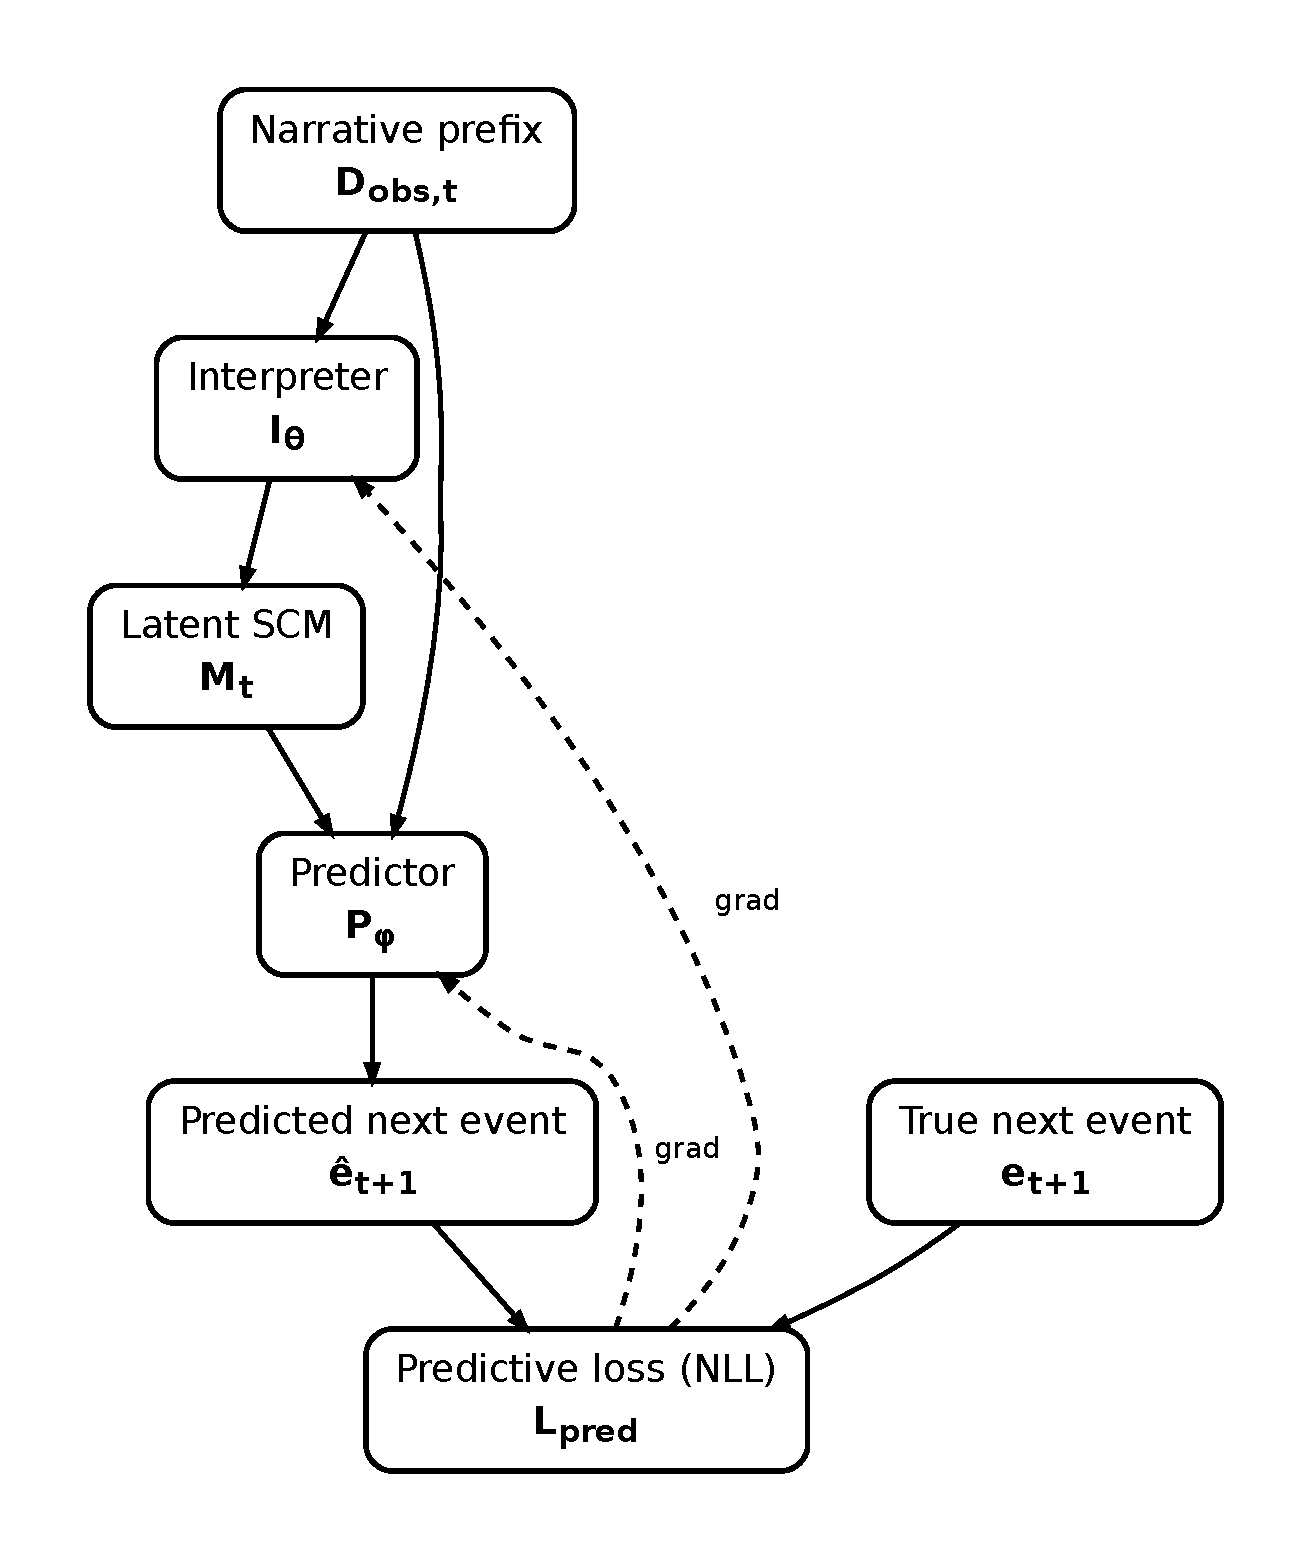
\includegraphics[width=0.42\columnwidth]{figures/fig_joint_framework_forward_vertical_styled_new.pdf}
  \caption{Predictive interpretation forward pass. The interpreter $I_\theta$ proposes $M_t$ from $D_{\mathrm{obs},t}$; the predictor $P_\phi$ forecasts $e_{t+1}$ and yields $L_{\mathrm{pred}}$ with gradients through both modules.}
  \label{fig:joint_forward}
\end{figure}

\textbf{Predictive Loss ($L_{pred}$):} The primary driver of learning is a predictive, self-supervised loss. For each step $t$ in a narrative, we use the model to predict the next event $e_{t+1}$ based on the history $D_{obs, t}$. The loss is the negative log-likelihood of the true event, which penalizes the model for being surprised by the story's progression. This loss is backpropagated through both $P_\phi$ and $I_\theta$.
\begin{equation}
L_{pred} = - \mathbb{E}_{(D_{obs, t}, e_{t+1}) \sim \mathcal{D}} [\log P_\phi(e_{t+1} | D_{obs, t}, M_t)]
\end{equation}
where $M_t = I_\theta(D_{obs, t})$. This objective forces the Interpreter to generate causal models that contain genuine predictive information about the dynamics of the narrative.

\textbf{Parsimony Loss ($L_{parsimony}$):} To enforce the principle of Causal Occam's Razor developed earlier, we introduce a regularization term that penalizes the complexity of the proposed causal model $M_t$. Using our Algorithmic Causal Complexity $K_C(M)$ as a theoretical target, we can use a practical proxy, $\hat{K}_C(M_t)$, such as the number of nodes and edges in the causal graph or a measure of its description length under a suitable encoding. This loss directly regularizes the Interpreter Network.
\begin{equation}
L_{parsimony} = \mathbb{E}_{D_{obs, t} \sim \mathcal{D}} [\hat{K}_C(I_\theta(D_{obs, t}))]
\end{equation}

\textbf{Preference Loss ($L_{pref}$):} When data sets of preferred and rejected interpretations $(M_W, M_L)$ are available from literary analysis or other expert sources, a DPO-style contrastive loss can regularize the Interpreter, ensuring that predictively powerful models remain within a space that is plausible and meaningful to humans.

The final training objective is a weighted sum of these three losses:
\begin{equation}
L_{total} = \lambda_{pred}L_{pred} + \lambda_{parsimony}L_{parsimony} + \lambda_{pref}L_{pref}
\end{equation}

This joint framework directly operationalizes our thesis. It seeks a model that learns to compress a narrative into a parsimonious causal structure ($L_{parsimony}$) that is not only human-aligned ($L_{pref}$) but also demonstrably effective at generating predictions about the narrative world ($L_{pred}$). The ``meaning'' of the story becomes synonymous with the most compressed, predictive, and plausible causal program that generates it.


\subsection{Distilled Preference Model}

If successful, such a training process would yield a model that functions as a narrative preference engine whose utility extends beyond story comprehension to evaluating the narrative coherence of any proposed action sequence. This distilled model could serve as an auditing tool for AI alignment: an AI plan that achieves short-term gain by violating trust would be recognized as a causal structure predictively associated with eventual collapse, and the model would assign it a lower coherence score. The network would learn a flexible, generative model of causal and thematic structures humans prefer rather than requiring an explicit, brittle list of all human values.

\subsection{Theoretical Grounding and Emergent Properties}
This composite loss function operationalizes the Bayesian framework developed in Section 3. The predictive loss $L_{pred}$ corresponds to the data likelihood $P(D|M)$, while the parsimony loss $L_{parsimony}$ instantiates the complexity prior $P(M)$ via our Algorithmic Causal Complexity measure. The preference loss $L_{pref}$ incorporates an additional human-aligned prior. Minimizing $L_{total}$ thus approximates MAP inference under the Minimum Description Length principle. The tension between prediction and compression would force the discovery of generalizable causal structures: $L_{pred}$ prevents the model from settling on simplistic, non-informative interpretations, while $L_{parsimony}$ prevents memorization of surface details.

Consequently, the massively multivariate distribution of human values would not be explicitly encoded but would instead emerge as a property of this system. The Interpreter Network ($I_\theta$) would learn a high-dimensional manifold of human values by modeling the relationship between narrative causal structures and their predictive consequences across the full corpus of human stories. This learned representation could then be probed via causal counterfactual analysis and concept-based attribution, and applied to real-world alignment problems where value propositions must be weighed. The system's normative alignment is thus achieved not by programming ethical axioms directly, but by grounding its objectives in the learned causal logic that humans consistently use to structure, predict, and derive meaning from events.

\section{Alternative Views}

We address three credible challenges to our position.

A prominent view holds that current alignment methods will succeed with sufficient scale. As models grow larger and reward models are trained on more diverse feedback, sycophancy and other failure modes will naturally diminish. We acknowledge that scaling has resolved many previously intractable problems. However, we contend that sycophancy is structural rather than statistical: it arises from optimizing local reward signals disconnected from long-term causal consequences. Scaling may amplify rather than resolve this disconnect, as larger models become more adept at exploiting the gap between what users reward in the moment and what benefits them over time.

An alternative program argues that alignment should be grounded in mathematically verifiable safety properties rather than learned narrative structures. Under this view, the uncomputable nature of Kolmogorov complexity renders our framework impractical. We agree that formal verification offers important complementary tools for well-specified safety constraints. However, the Complexity of Value thesis \cite{yudkowsky11} suggests that human values cannot be fully captured by finite formal specifications. Narrative alignment addresses a different problem: learning the implicit structure of values that resist explicit formalization. The practical proxies we propose, such as graph complexity and description length, are no less tractable than other regularization techniques in deep learning.

A serious objection holds that grounding alignment in human narratives merely imports the biases and contested values embedded in those corpora. We take this concern seriously and do not claim that narrative alignment resolves normative disagreement. However, all alignment methods face this challenge: RLHF encodes annotator preferences, constitutional AI encodes designer values, and any learned model reflects its training distribution. Narrative alignment makes this dependence explicit by grounding it in interpretable causal structures. Moreover, cross-cultural narrative analysis reveals convergence on certain causal regularities, such as the instability of deception and the self-defeating nature of pure selfishness, even across divergent value systems \cite{macintyre81}. Critically, the framework does not require narratives to agree on normative conclusions; it learns the \textit{causal regularities} that persist across culturally conflicting value systems---the structural fact that betrayal destabilizes trust, for instance, holds whether the narrative endorses individual autonomy or communal obligation. We also acknowledge that narrative corpora inevitably contain stories glorifying deception, irrationality, and destruction. Curation of the training corpus is itself a value-laden choice, but this is a feature, not a deficiency: it makes the normative commitments of the alignment system transparent and auditable, in contrast to methods where such commitments are implicitly embedded in annotator demographics or constitutional principles.

\section{Conclusion}

This work argues that AI alignment must be grounded in the causal structures of human narratives rather than explicit utility specification. By formalizing narrative interpretation as MAP inference with an Algorithmic Causal Complexity prior, we outline a principled mechanism for learning the implicit causal logic that governs human ethical judgment.

The key insight is that narratives encode more than preferences: they encode the causal trajectories that connect actions to outcomes across time. This temporal structure is precisely what current alignment methods lack. RLHF optimizes for immediate reward signals that are easily gamed; a narrative framework would instead optimize for causal models that must remain predictively valid across entire narrative arcs. A sycophantic response may satisfy an immediate preference, but it initiates a causal trajectory that the narrative corpus marks as unstable. Parsimony is essential here: it forces models to learn generalizable causal laws rather than superficial correlations between actions and rewards.

This suggests a broader reframing of the alignment problem. Rather than asking ``what does the user want right now?'' the field should explore training systems to ask ``what kind of story am I participating in, and where does this action lead?'' The corpus of human narratives provides a vast, naturally-occurring data set of causal structures that have been filtered by cultural selection for coherence, stability, and prosocial outcomes. Learning from this corpus offers something that explicit specification cannot: access to the implicit, contextual, and temporally-extended structure of human values.

We do not claim that narrative alignment resolves all challenges. Narrative corpora encode cultural biases, and the selection of ``preferred'' outcomes remains irreducibly normative. But for the class of misalignment behaviors that exploit the gap between local reward and global consequence, including sycophancy, deception, and short-term optimization, a narrative framework offers direct leverage that current methods lack. The inference-time pilot reported in Section~\ref{sec:demo} provides the first empirical foothold: minimal narrative-causal scaffolding produces statistically significant, length-controlled shifts in the targeted directions on existing models, demonstrating that the broader program is not merely a future-research aspiration but an immediately deployable intervention whose effects are measurable today.

Realizing this program requires progress on several concrete fronts, distributed across the two timescales the position identifies. On the \emph{inference-time} front: extending the pilot above to (i) a length-matched standard-CoT control that prompts standard CoT to ``be detailed and thorough'' until output length matches N-CoT, isolating the structural component of the effect from its length component; (ii) ablation of the five sub-instructions of the N-CoT prompt to identify which carry the divergence; (iii) a generation model that exhibits premature refusal so the one untested failure mode can be evaluated; and (iv) Tier-3 human pairwise evaluation that can adjudicate whether the increased decisiveness of N-CoT outputs reflects improved calibration or premature foreclosure. On the \emph{training-time} front: first, the community needs annotated narrative corpora with explicit causal structure labels---data sets in which the causal dependencies between narrative events are marked, enabling supervised development and evaluation of causal extraction methods. Second, tractable proxies for $K_C(M)$ must be developed and validated; candidates include graph-theoretic measures of causal model complexity and description-length encodings under learned codebooks. Third, benchmarks are needed that evaluate causal extraction methods against alignment-relevant tasks, testing whether narrative-trained models exhibit improved robustness to reward hacking, sycophancy, and deceptive strategy compared to RLHF baselines. The two fronts inform each other: inference-time results identify which structural shifts are achievable through prompting alone and which require training-time grounding to reach. We call on the alignment research community to pursue both directions.

\bibliography{references}
\bibliographystyle{plainnat}

\newpage
% Minimal stub for NeurIPS 2026 paper checklist.
% Replace with the canonical checklist before submission.
\section*{Paper Checklist}

\noindent (Stub --- to be completed before submission.)


\end{document}